
As Figuras \ref{fig:tr2-1n} e \ref{fig:tr2-2n} apresentam os gráficos com a curva ajustada para o período de retorno de 2 anos e 1 ou 2 neurônios na rede.

%TR 2
\begin{figure}[H]
    \caption{Curva ajustada para os dados para TR 2 anos e 1 neurônio artificial}
    \centering
    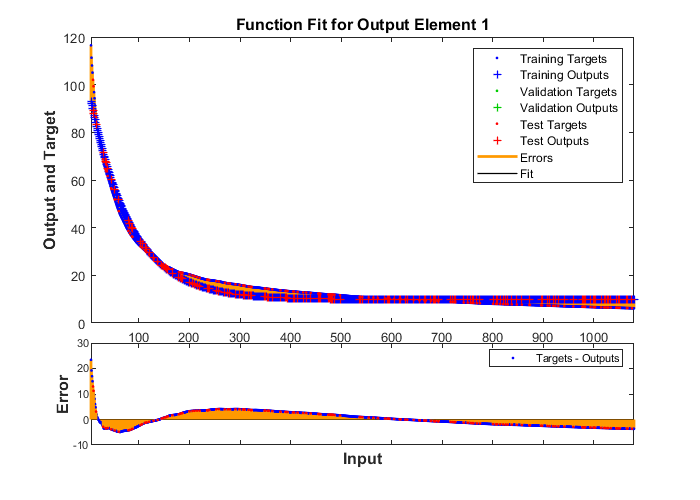
\includegraphics[width=0.74\textwidth]{Textuais/Figuras/NN/tr2-1neuronio.png}
    \fonte{Autores}
    \label{fig:tr2-1n}
\end{figure}


\begin{figure}[H]
    \caption{Curva ajustada para os dados para TR 2 anos e 2 neurônios artificiais}
    \centering
    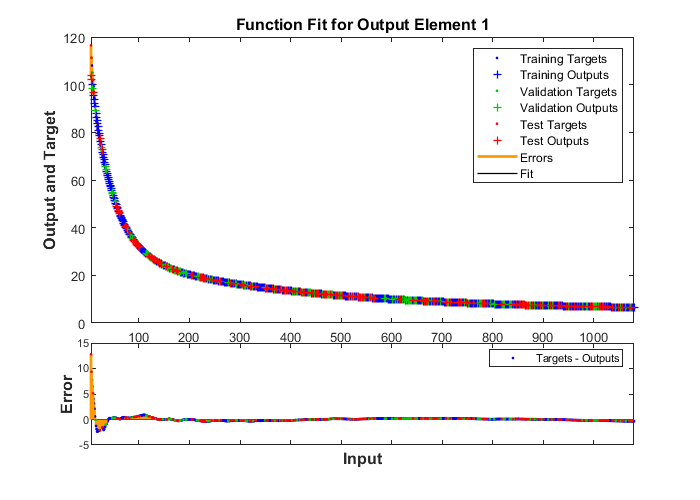
\includegraphics[width=0.74\textwidth]{Textuais/Figuras/NN/tr2-2neuronio.png}
    \fonte{Autores}
    \label{fig:tr2-2n}
\end{figure}

\begin{figure}[H]
    \caption{Curva ajustada para os dados para TR 2 anos e 5 neurônios artificiais}
    \centering
    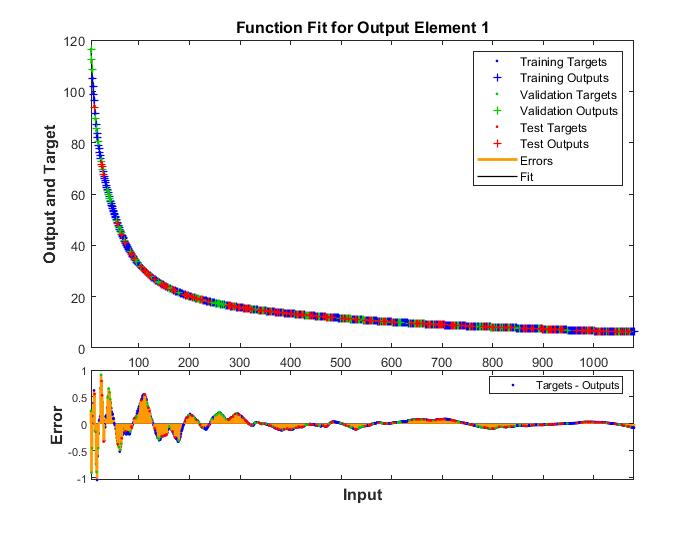
\includegraphics[width=0.74\textwidth]{Textuais/Figuras/NN/tr2-5neuronio.png}
    \fonte{Autores}
    \label{fig:tr2-5n}
\end{figure}

\begin{figure}[H]
    \caption{Curva ajustada para os dados para TR 2 anos e 10 neurônios artificiais}
    \centering
    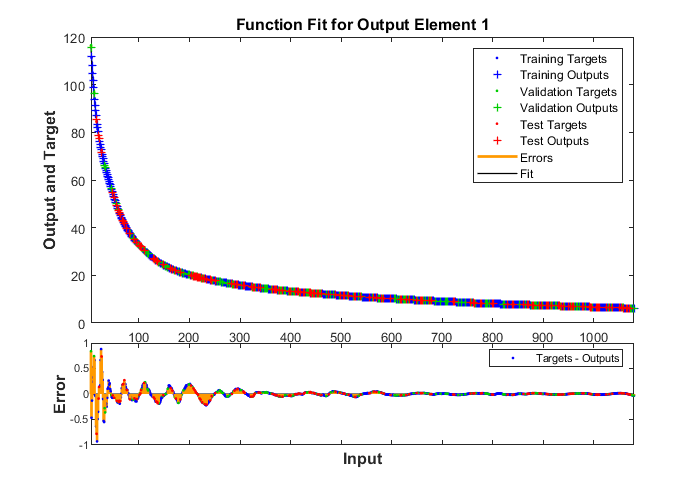
\includegraphics[width=0.74\textwidth]{Textuais/Figuras/NN/tr2-10neuronio.png}
    \fonte{Autores}
    \label{fig:tr2-10n}
\end{figure}
%FIM TR 2

\begin{figure}[H]
    \caption{Comparação entre as curvas geradas para TR2 e 10 neurônios}
    \centering
    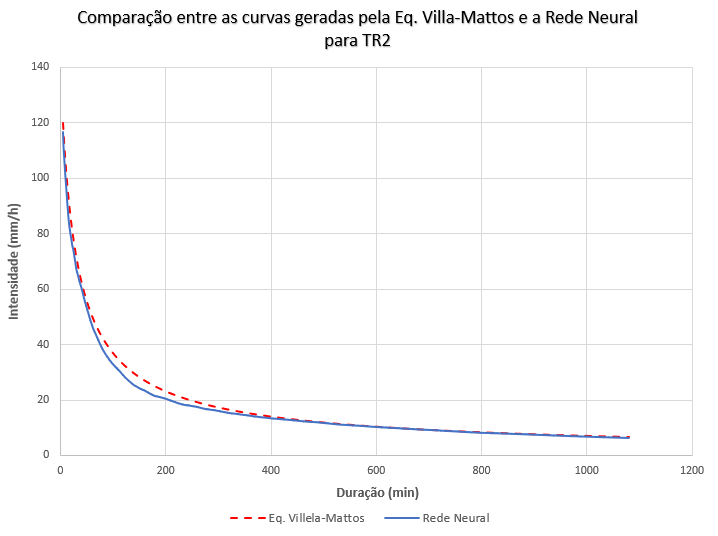
\includegraphics[width=\textwidth]{Textuais/Resultados/Comparacao/TR2.png}
    \fonte{Autores}
    \label{fig:comp-tr2}
\end{figure}